\subsection{Accelerometeralgoritme}

For at teste, om omregningen fra spændingen til vinkler fungerer i praksis, bevæges vinkeltesteren, der er vist på \autoref{fig:vinkeltest}, fra $180^{\circ}$ til $70^{\circ}$. 
Figur \ref{fig:spaending_vinkel_test} illustrerer dette i MATLAB, hvor vinklen er illustreret på den venstre Y-akse, og hvor accelerometrenes spænding er illustreret på den højre Y-akse.

\begin{figure}[H]
\centering
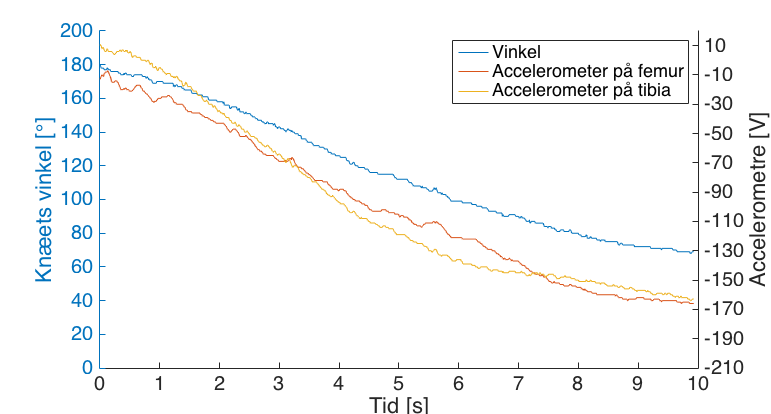
\includegraphics[width=1\textwidth]{figures/spaending_vinkel_test}
\caption{Test af vinkelberegning. Vinklen, som er den blå graf, er svarende til den samlede vinkel mellem de to accelerometre, hvor værdierne er illustreret på Y-aksen til venstre i grader. Spændingen målt for de to accelerometre måles i forhold til Y-aksen til højre og er vist ved en rød og gul graf.}
\label{fig:spaending_vinkel_test}
\end{figure}

\noindent
Det ses på \autoref{fig:spaending_vinkel_test}, at der er en sammenhæng mellem spænding fra accelerometrene og den samlede vinkel over knæleddet. 
Der tages udgangspunkt i \autoref{tab:vinkelinterval_psoc} for omregningen, hvoraf spændingen for hvert accelerometer omregnes til grader. 
Disse lægges sammen for at udregne den samlede vinkel. 
Derudover illustrerer figuren, at vinklerne virker inden for det forventede arbejdsområde på $90$-$180^{\circ}$, dertil kan vinklen over knæet ligeledes bestemmes under $90^{\circ}$. 
På figuren aflæses, at systemet registrerer en vinkel på $90^{\circ}$, når  accelerometeret på femur giver en spænding på $-0,2191~V$ og accelerometeret på tibia giver en spænding på $-0,2336~V$. 

For at teste vinkelberegningen sammenlignes de målte spændinger for accelerometrene, der er illustreret på \autoref{fig:spaending_vinkel_test}, og de konverterede digitale outputværdier i \autoref{sec:imp_vinkler}, der er omregnet til en tilsvarende spænding. 
De omregnede spændinger fra accelerometrene er lagt sammen for at få den samlede spænding, der opnås ved en tilsvarende vinkel. 
Resultaterne heraf fremgår på \autoref{tab:vinkel_test_afvigelse}.

\begin{table}[H]
\centering
\begin{tabular}{|c|c|c|c|}
\hline
\textbf{Vinkel {[}{$^{\circ}$}{]}} & \textbf{Implementeret spænding {[}V{]}} & \textbf{Målt spænding {[}V{]}} & \textbf{Afvigelse {[}\%{]}} \\ \hline
\textbf{180}                    & 0                         & -0,00323                       & 0,3                      \\ \hline
\textbf{160}                    & -0,1136                   & -0,11118                       & 2,1                       \\ \hline
\textbf{140}                    & -0,2150                   & -0,2240                        & 4,2                   \\ \hline
\textbf{100}                    & -0,4044                   & -0,4109                        & 1,6                    \\ \hline
\textbf{80}                     & -0,5447                   & -0,4906                        & 3,4                    \\ \hline
\end{tabular}
\caption{Udregnede afvigelser mellem de implementerede og målte spændinger inddelt efter vinkler på henholdsvis $180$, $160$, $140$, $100$ og $80^{\circ}$. Det fremgår, at afvigelsen er mellem $0,3$ til $4,2~\%$.}
\label{tab:vinkel_test_afvigelse}
\end{table}

\noindent
Ud fra \autoref{tab:vinkel_test_afvigelse} fremgår en afvigelse mellem $0,3$ og $4,2~\%$. Spændingen for de $80^{\circ}$ er beregnet ud fra et interval mellem $60$ og $100^{\circ}$, hvilket er et interval på $40^{\circ}$. Vinklerne, der er udregnet ud fra et interval på $40^{\circ}$, herunder vinkler på henholdsvis $80$ og $100^{\circ}$, har en højere afvigelse end de vinkler, hvor spændingen er udregnet ud fra et interval på $20^{\circ}$. 


Vinklen på $80^{\circ}$ har ikke en betydning, da systemet er designet til at fungere inden for $90$ til $180^{\circ}$.
Det vurderes, at afvigelsen ikke har den store betydning for det samlede system, da $80^{\circ}$ ligger uden for intervallet på $90$ til $180^{\circ}$. 
Derudover er systemets primære opgave at signalere, når knæets vinkel er under $90^{\circ}$ eller over $180^{\circ}$ ved en rød LED, hvorfor $140^{\circ}$ ikke vil have en betydning for dette. Af denne grund godkendes  afvigelsen ved disse grader. 

For at teste, hvorvidt LED'en på mikrokontrolleren signalerer når en vinkel mellem $90$ og $180^{\circ}$ overskrides, anvendes vinkeltesteren fra pilotforsøget, der ses på \autoref{fig:vinkeltest}. Vinkeltesteren indstilles til henholdsvis $40^{\circ}$, $100^{\circ}$ og $200^{\circ}$. 
Heraf ses, at LED'en lyser grønt ved de acceptable vinkler mellem $90-180^{\circ}$, og rødt ved vinkler udenfor dette interval. Dette ses på \autoref{fig:mikro_LED}.

\begin{figure}[H]
\centering
\includegraphics[width=1\textwidth]{figures/mikro_LED}
\caption{Mikrokontrollerens LED ses lyse grøn indenfor $90-180^{\circ}$ og lyse rød ved vinkler udenfor.}
\label{fig:mikro_LED}
\end{figure}

\noindent
Ved en overskridelse af grænsen for vinklen, skal det ligeledes visualiseres. 
Der er foretaget en test, hvor accelerometrene er påsat en forsøgsperson, som først overstrækker knæleddet, og derefter udfører en squat-øvelse. 
En visualisering heraf ses af \autoref{fig:vinkeltest_graenser}.

\begin{figure}[H]
\centering
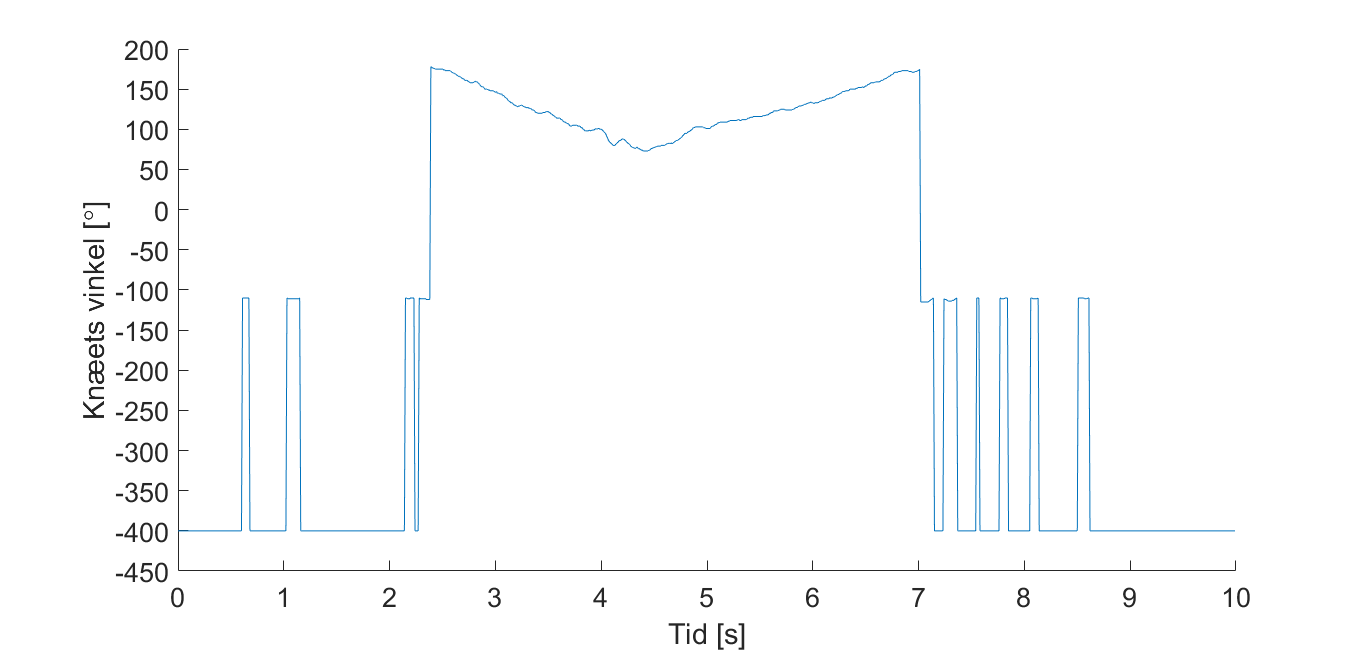
\includegraphics[width=1\textwidth]{figures/vinkeltest_graenser}
\caption{Grafen illustrerer vinklen over knæet under en squat-øvelse. En vinkel under $-100^{\circ}$ symboliserer en overskridelse af $180^{\circ}$ over knæleddet.}
\label{fig:vinkeltest_graenser}
\end{figure}

\noindent
Det ses på \autoref{fig:vinkeltest_graenser}, at forsøgspersonen overstrækker knæleddet de første $2~s$, således begge accelerometre overstiger grænsen på $90^{\circ}$, der tilsammen udgør en vinkel på $180^{\circ}$. 
Dette visualiseres ved en vinkel på $-400^{\circ}$. 
Efter 0,5 sekunder ses en vinkel på $-110^{\circ}$, hvilket er gældende, da det ene accelerometer har haft en spænding svarende til præcis $90^{\circ}$ og har derfor ikke overskredet grænsen. 
Ved squat-øvelsens begyndelse falder vinklen fra $180$ til $73^{\circ}$, hvorefter den stiger til $180^{\circ}$. 
Til slut i målingen ses igen et fald under $-100^{\circ}$, hvilket indikerer, at forsøgspersonen igen overstrækker knæleddet.

\noindent
En yderligere test er foretaget for at undersøge forsinkelsen, og følger samme anvisninger beskrevet i \autoref{sec:lavpas_test}.  
Resultatet af denne test giver en forsinkelse på  $3,6~\mu s$. Dette betragtes ikke som værende af signifikant betydning i forhold til det samlede system, hvorfor denne forsinkelse accepteres.


\vspace{3mm}
\textbf{Opsummering af krav:}
\begin{itemize}
%\item[\text{\sffamily \checkmark}] Skal kunne udregne en samlet vinkel over knæet
\item[\text{\sffamily \checkmark}] Skal kunne udregne knæets vinkel indenfor intervallet $90-180^{\circ}$
\begin{itemize}
\item Dette skal indikeres ved en grøn LED
\end{itemize}
\item[\text{\sffamily \checkmark}] Skal indikere, hvornår knæets vinkel er udenfor intervallet $90-180^{\circ}$
\begin{itemize}
\item Dette skal indikeres ved en rød LED
\item Hvis vinklen for ét accelerometer overstiger $90^{\circ}$, indikeres dette som et output på $-200^{\circ}$, hvortil det andet accelerometers vinkel lægges til de $-200^{\circ}$
\item Hvis vinklen overstiger $90^{\circ}$ for hvert accelerometer, skal dette indikeres som et output på $-400^{\circ}$
\end{itemize}
\end{itemize}